\section{Grundlagen}

\subsection{Überblick}
Um unseren Lösungsansatz nachvollziehen zu können, ist es erforderlich, 
die Problemstellung detailliert zu analysieren. Im ersten Schritt wird betrachtet, 
welche Zielgruppe Ludwig System anspricht und welche spezifischen Optimierungen 
das Unternehmen verfolgt. Im Anschluss werden bestehende Lösungsansätze verglichen, 
um deren Stärken und Schwächen zu bewerten und als Grundlage 
für die Entwicklung eines verbesserten Systems zu nutzen.

\subsubsection{Anwendungsdomäne}
Das Abhängen von Lasten per Hand ist nicht nur zeitaufwendig, sondern oft auch gefährlich. 
Ludwig System bietet mit ihren funkgesteuerten Lasthaken eine innovative Lösung, 
die diese Arbeit deutlich erleichtert. Diese Haken ermöglichen es den Mitarbeitenden, 
Lasten aus sicherer Entfernung anzuheben und auszubalancieren. Besonders beliebt ist 
die Traverse, die speziell für den Transport von Dachelementen und Wänden entwickelt wurde. 
Allerdings müssen aktuelle Versionen noch manuell an die Last befestigt werden, 
was besonders bei hohen Wänden zeitaufwendig und gefährlich sein kann. 
Abbildung 2.2 illustriert die Nutzung der Traverse beim Transport eines Dachelements.

\begin{figure}[H]
    \centering
    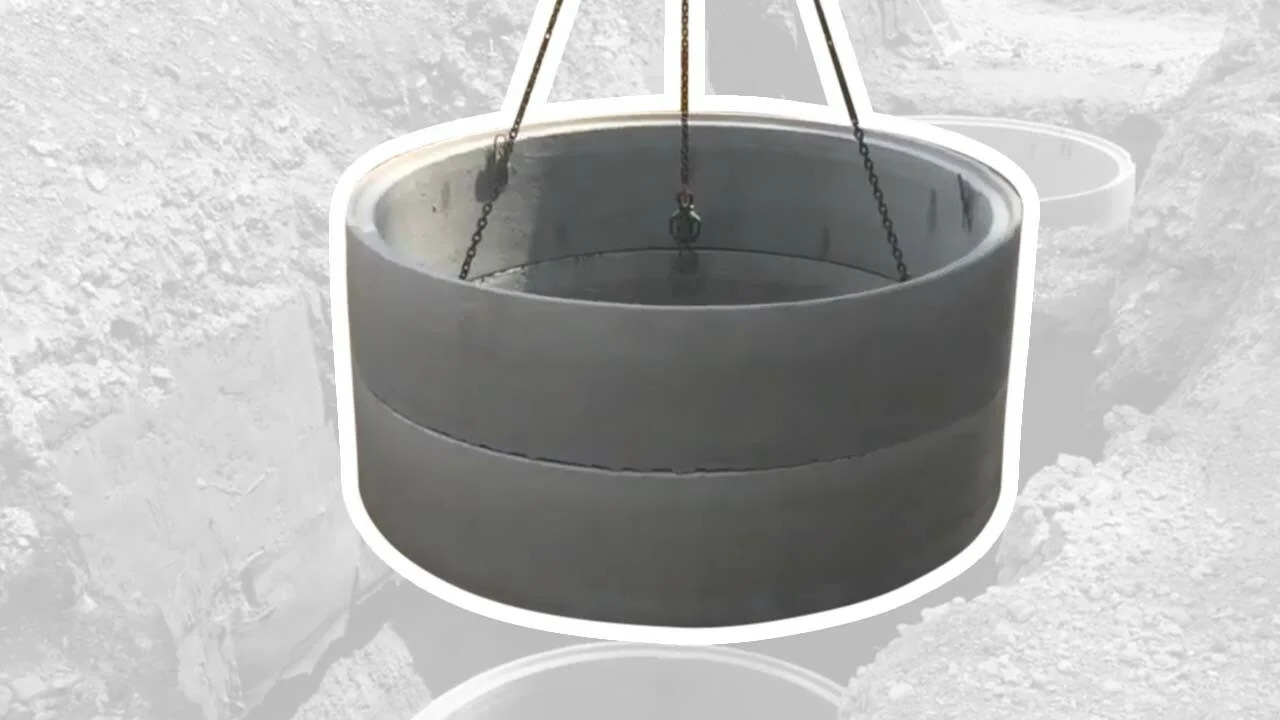
\includegraphics[width=0.5\textwidth]{graphics/Betonelement.jpg}\hfill%
    \caption{Ludwig Hook mit Betonelement}
    \centering
    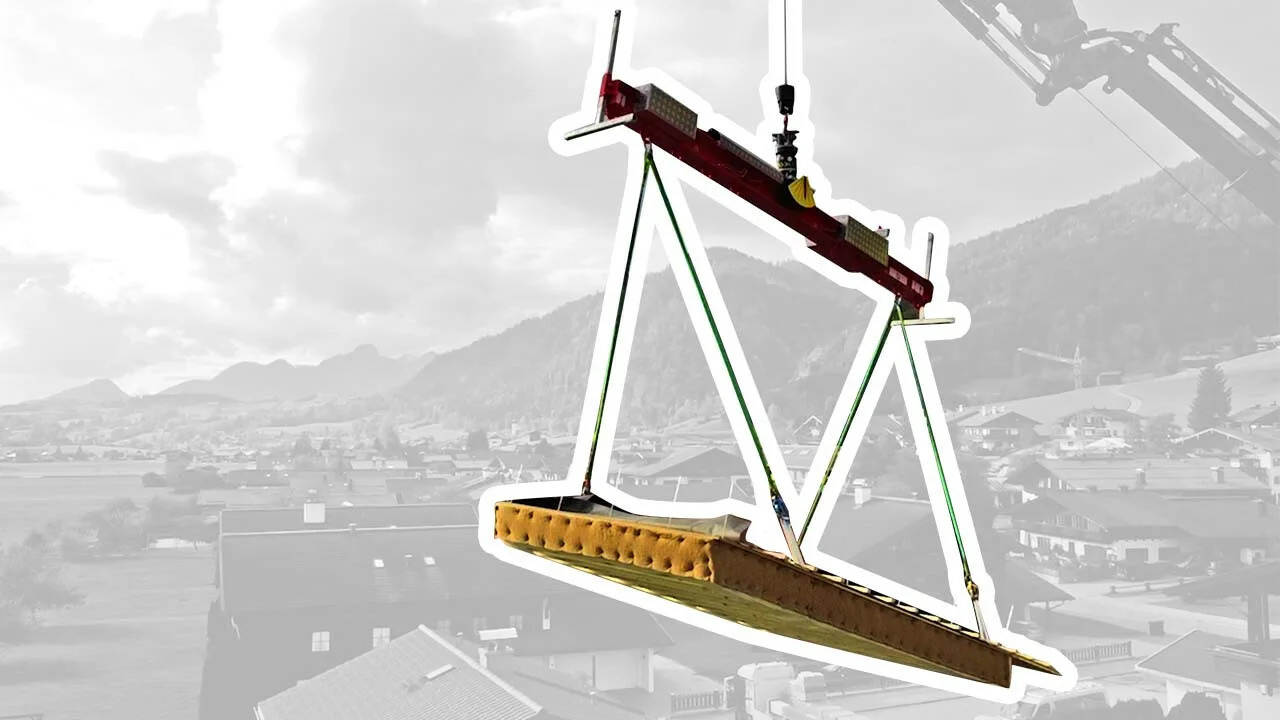
\includegraphics[width=0.5\textwidth]{graphics/Traverse.jpg}
    \caption{Traverse mit Dachelement}
\end{figure}

\subsubsection{Last}
Unter Lasten sind vor allem Fertigstrukturen wie z.B. Fertig erstellte Wände oder Dächer. 
Lasten haben maximal 2 Anschlagspunkte, welche einen Abstand von 1m bis 6m zueinander haben.
Diese Anschlagspunkte können auf unterschiedliche Höhen sein, wie z.B. bei Dächern welche eine
Neigung besitzen.

\clearpage
\subsubsection{Traverse}
Die LudwigTraverse ist eine Spezialtraverse, die speziell für den Lastausgleich entwickelt 
wurde. Sie erweist sich insbesondere dann als nützlich, wenn die Anschlagspunkte 
falsch positioniert sind und dadurch der Schwerpunkt der Last nicht korrekt berücksichtigt wird. 
Dies kann zu einer schrägen Ausrichtung beim Anheben der Last führen \cite{ludwigTraverse}.

\begin{figure}[H]
    \centering
    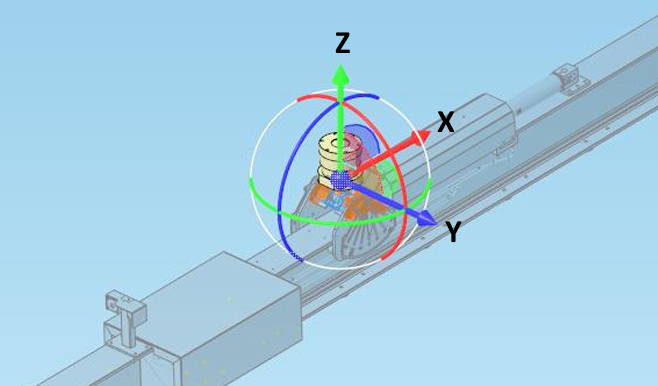
\includegraphics[width=0.5\linewidth]{graphics/Traverse_Rotationen.PNG}
    \caption{Koordinatensystem der Ludwig System Traverse}
    \label{fig:traverse}
\end{figure}

Abbildung \ref{fig:traverse} zeigt das linkshändige Koordinatensystem der Traverse.
Die Traverse hat Dimensionen (Länge × Breite × Höhe) von 500 cm × 70 cm × 50 cm.
Dabei wird fortan die Rotation um die Y-Achse der Traverse als Neigen definiert und die Rotation 
um die Z-Achse der Traverse als Rotieren definiert.

\subsection{Stand der Forschung}

\subsubsection{Arbeit: Objekterkennung und Distanzmessung für Kollisionsvermeidung bei Lastenhebung}
(Arbeit: Object Detection and Distance Measurement Algorithm for Collision Avoidance of Precast Concrete Installation during Crane Lifting Process\cite{yong_object_2023} Erklären)

\subsubsection{Arbeit: Objekterkennung und 3D-basierte Objektortung für automatische Lastenhebung}
(Arbeit: Image-based onsite object recognition for automatic crane lifting tasks\cite{zhou_image-based_2021} Erklären)

\subsubsection{Arbeit: Erkennung von auf Robotersystemen angebrachten Passermarken}

\clearpage
\subsection{Passermarker}
Passermarker sind ein essenzielles Werkzeug in der modernen Bildverarbeitung und spielen eine 
zentrale Rolle in der räumlichen Orientierung und Positionsbestimmung. Insbesondere in Anwendungen 
wie der automatisierten Lastenhebung, wie sie von Ludwig System angestrebt wird, können Passermarker 
helfen, Anschlagpunkte präzise zu lokalisieren.

Diese Marker, darunter Barcodes, QR-Codes oder speziell entwickelte AR-Marker, liefern visuelle 
Referenzen, die von Kamerasystemen erkannt und interpretiert werden können. Damit ermöglichen sie es, 
Objekte im Raum genau zu positionieren oder auszurichten.

In diesem Abschnitt untersuchen wir die Grundlagen von Passermarkern und beleuchten ihre spezifischen 
Einsatzmöglichkeiten in unserem Szenario, insbesondere im Kontext der automatisierten Ausrichtung von 
Anschlagpunkten auf der Traverse.

\subsubsection{Einführung Passermarker}
Passermarker sind quadratische Muster, die auf flachen Oberflächen aufgedruckt werden. 
Sie dienen als visuelle Referenzpunkte, die von Kamerasystemen erkannt und interpretiert 
werden können. Es gibt verschiedene Arten von Passermarkern, die je nach Anwendung 
unterschiedliche Eigenschaften und Einsatzmöglichkeiten bieten. 
Abbildung \ref{fig:marker_types} zeigt eine Auswahl solcher Marker.

\begin{figure}[H]
    \centering
    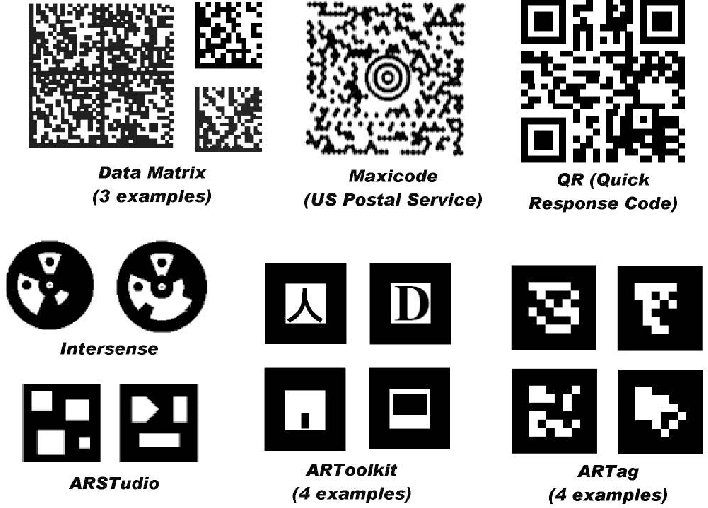
\includegraphics[width=0.5\linewidth]{graphics/marker_arten.png}
    \caption{Verschiedene Markerarten}
    \label{fig:marker_types}
\end{figure}

Grundsätzlich gilt: Je komplexer und grösser ein Marker ist, desto mehr Informationen können
darin gespeichert werden. Dabei muss jedoch der Informationsgehalt immer an die spezifischen 
Anforderungen der Anwendung angepasst werden, um eine optimale Balance zwischen Grösse, Lesbarkeit 
und Informationsdichte zu gewährleisten.

In der Robotik gehören AprilTags und AruCo-Marker zu den meistgenutzten Passermarkern. 
Ihre Beliebtheit basiert auf ihrer Robustheit und Effizienz bei der Lokalisierung in 
dreidimensionalen Räumen. Diese Marker wurden speziell entwickelt, um Verzerrungen und 
schwierige Lichtverhältnisse zu kompensieren und eine präzise Posenschätzung zu ermöglichen. 
Ihre Anwendung wird im weiteren Verlauf dieser Arbeit genauer beleuchtet, insbesondere im 
Kontext der automatisierten Lokalisierung von Anschlagpunkten.
\clearpage
\subsubsection{Posenschätzung durch AR Marker}
Das Problem der Posenberechnung stammt aus dem Bereich der erweiterten 
Realität. Dabei wird eine Gleichung gelöst, die den Projektionsfehler 
zwischen den 2D-Bildpunkten und den 2D-Projektionen der 3D-Weltpunkte minimiert. 
Das Lösen dieser Gleichung liefert einen Rotations- und Translationsvektor, der 
die Position und Orientierung der Kamera im Koordinatensystem beschreibt. 
Abbildung \ref{fig:pose} illustriert diesen Zusammenhang.

\begin{figure}[H]
    \centering
    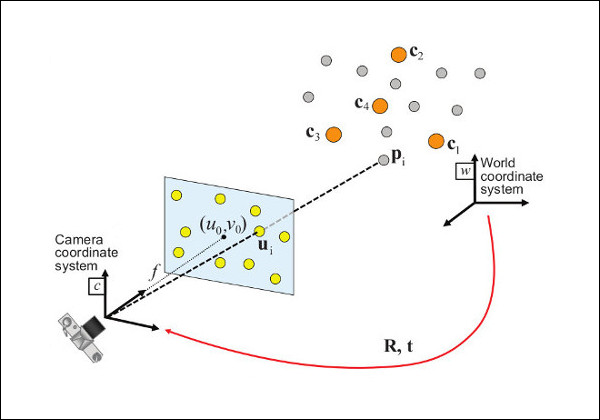
\includegraphics[width=0.4\linewidth]{graphics/pose.png}
    \caption{Posenschätzung}
    \label{fig:pose}
\end{figure}

Laut \cite{pose} braucht es dazu folgende Komponenten: die intrinsischen Parameter 
der Kamera \( K \) und die Projektionsmatrix \( \Pi \). Die intrinsischen Parameter 
können bereits vorher durch die Kalibrierung der Kamera berechnet werden. Die Kalibrierung 
wird mit OpenCV-Methoden durchgeführt, wie in \cite{zhang} und \cite{bradski} detailliert 
beschrieben.

Mithilfe der beiden Matrizen lässt sich eine Gleichung aufstellen, die \( N \) Punkte 
in der 3D-Welt auf 2D-Bildpunkte projiziert. Dabei entstehen die Rotationsmatrix und der 
Translationsvektor, die in der Transformationsmatrix \({}^{c}\mathbf{T}_{w}\) enthalten sind.
Mit der Schätzung dieser Matrix können Weltkoordinaten in Kamerakoordinaten transformiert 
werden.

Gleichung um Weltkoordinaten im Bild zu projizieren:
\[
\begin{bmatrix}
u \\ 
v \\ 
1
\end{bmatrix}
=
\mathbf{A} \mathbf{\Pi} {}^{c}\mathbf{T}_{w}
\begin{bmatrix}
X_w \\ 
Y_w \\ 
Z_w \\ 
1
\end{bmatrix}
\]

\[
\begin{bmatrix}
u \\ 
v \\ 
1
\end{bmatrix}
=
\begin{bmatrix}
f_x & 0   & c_x & 0 \\ 
0   & f_y & c_y & 0 \\ 
0   & 0   & 1   & 0
\end{bmatrix}
\begin{bmatrix}
1 & 0 & 0 & 0 \\ 
0 & 1 & 0 & 0 \\ 
0 & 0 & 1 & 0
\end{bmatrix}
\begin{bmatrix}
r_{11} & r_{12} & r_{13} & t_x \\ 
r_{21} & r_{22} & r_{23} & t_y \\ 
r_{31} & r_{32} & r_{33} & t_z \\ 
0      & 0      & 0      & 1
\end{bmatrix}
\begin{bmatrix}
X_w \\ 
Y_w \\ 
Z_w \\ 
1
\end{bmatrix}
\]

Gleichung um Weltkoordinaten in Kamerakoordinaten zu transformieren:

\[
\begin{bmatrix}
X_c \\ 
Y_c \\ 
Z_c \\ 
1
\end{bmatrix}
=
{}^{c}\mathbf{T}_{w}
\begin{bmatrix}
X_w \\ 
Y_w \\ 
Z_w \\ 
1
\end{bmatrix}
\]

\[
\begin{bmatrix}
X_c \\ 
Y_c \\ 
Z_c \\ 
1
\end{bmatrix}
=
\begin{bmatrix}
r_{11} & r_{12} & r_{13} & t_x \\
r_{21} & r_{22} & r_{23} & t_y \\
r_{31} & r_{32} & r_{33} & t_z \\
0 & 0 & 0 & 1
\end{bmatrix}
\begin{bmatrix}
X_w \\ 
Y_w \\ 
Z_w \\ 
1
\end{bmatrix}
\]

\subsubsection{Probleme mit Passermarkern}
Mithilfe von Passermarkern können wir Anschlagpunkte erkennen und dessen Position bestimmen.
Zusätzlich können wir mit deren Hilfe ausrechnen wie sich die Traverse Positionieren musss, damit
sich über den den Anschlagspunkten befindent.

Allerdings stellen Passsermarker keine perfekte Lösung dar, um Anschlagpunkte zuverlässig zu lokalisieren. 
Sie sind besonders empfindlich gegenüber äusseren Einflüssen. Bereits geringe Verschmutzungen, 
wie etwa Schmutz oder Staub auf den Kanten, können die Erkennung erheblich beeinträchtigen 
oder sogar vollständig verhindern.

Darüber hinaus sind Passermarker anfällig für ungünstige Lichtverhältnisse. Blendung, Schatten 
oder Reflexionen können die Erkennungsrate deutlich verringern, insbesondere in Aussenbereichen 
oder bei wechselnden Lichtbedingungen. Auch der Erkennungsbereich der Marker ist begrenzt: Marker 
müssen sich in einem bestimmten Abstand und Winkel zur Kamera befinden um erkannt zu werden.

Grössere Marker können zwar leichter erkannt werden, bringen jedoch eigene Herausforderungen mit sich. 
insbesondere wenn auf der Last nicht genügend Platz für die Anbringung verfügbar ist. Zudem nutzen 
sich Marker durch äussere Einflüsse, wie Witterung oder mechanische Belastung, schnell ab. Um die 
Erkennung dauerhaft zu gewährleisten, müssen sie regelmässig ersetzt oder neu angebracht werden.



\subsection{Objekterkennung durch Machine Learning}
Künstliche Intelligenz (KI) spielt eine immer wichtigere Rolle in verschiedenen Bereichen 
unseres Lebens und wird auch in Zukunft zahlreiche Innovationen vorantreiben. 
Bereits heute revolutioniert sie viele Branchen, darunter die Automatisierung, 
Bildverarbeitung und Robotik. Eine besonders relevante Disziplin innerhalb der KI ist die 
Objekterkennung, die mithilfe von neuronalen Netzen umgesetzt wird.

Speziell für die vorliegende Problemstellung könnte eine KI entwickelt werden, die in der 
Lage ist, Anschlagpunkte unterschiedlicher Arten präzise zu erkennen und zu markieren. 
Durch den Einsatz von Machine-Learning-Modellen kann die Erkennung kontinuierlich verbessert 
werden, indem sie aus neuen Daten lernt und sich an verschiedene Szenarien und Bedingungen 
anpasst.

\subsubsection{Grundlagen Objekterkennung mit Neuronalen Netzen}
Neuronale Netzwerke sind inspiriert vom menschlichen Gehirn, bei dem Informationen zwischen Neuronen weitergegeben 
werden. Dabei verarbeitet jedes Neuron Signale und leitet sie verstärkt oder abgeschwächt an das nächste Neuron weiter.
Abbildung \ref{fig:humanCell} zeigt eine schematische Darstellung, wie Neuronen im menschlichen Gehirn miteinander 
kommunizieren.

\begin{figure}[H]
    \centering
    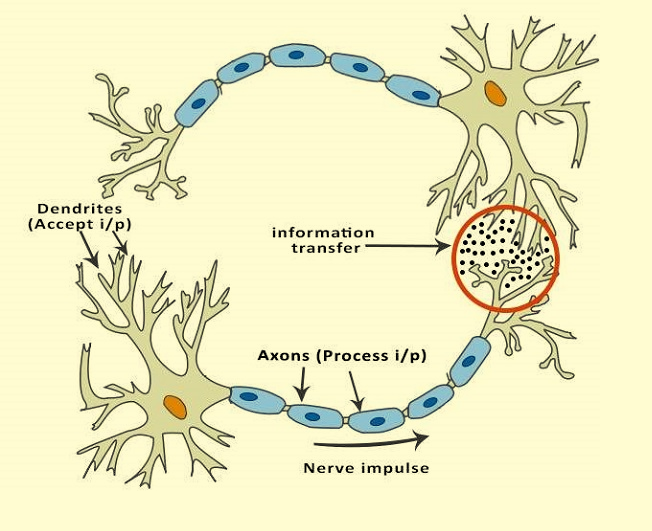
\includegraphics[width=0.4\linewidth]{graphics/human_model.png}
    \caption{Biologisches Neuron im menschlichen Gehirn}
    \label{fig:humanCell}
\end{figure}

Ähnlich wie das menschliche Gehirn Muster wie Kanten und Farben erkennen kann, werden künstliche neuronale Netzwerke 
darauf trainiert, Muster in numerischen Daten zu identifizieren. Maschinen sehen jedoch keine Bilder direkt, sondern 
verarbeiten Zahlenwerte (z. B. Pixelintensitäten), die aus den Bildern extrahiert werden. Dazu benötigen neuronale 
Netzwerke Parameter, die während des Trainingsprozesses optimiert werden. Zusätzlich wird ein Fehlersignal berechnet, 
wenn das Modell falsche Vorhersagen trifft, um das Lernen zu steuern.

Abbildung \ref{fig:network} zeigt die Struktur eines neuronalen Netzwerks mit drei Schichten: der Eingabeschicht (Input Layer), 
den verborgenen Schichten (Hidden Layers) und der Ausgabeschicht (Output Layer). Im Input Layer werden die Pixelwerte 
eines Bildes verarbeitet. Diese Werte werden mit den Gewichten der Verbindungen zwischen den Neuronen multipliziert, 
aufsummiert und an die nächste Schicht weitergegeben. In den Hidden Layers werden diese Berechnungen weitergeführt, 
bis im Output Layer eine Wahrscheinlichkeitsverteilung ausgegeben wird, die anzeigt, ob ein Anschlagspunkt im Bild 
vorhanden ist.

\begin{figure}[H]
    \centering
    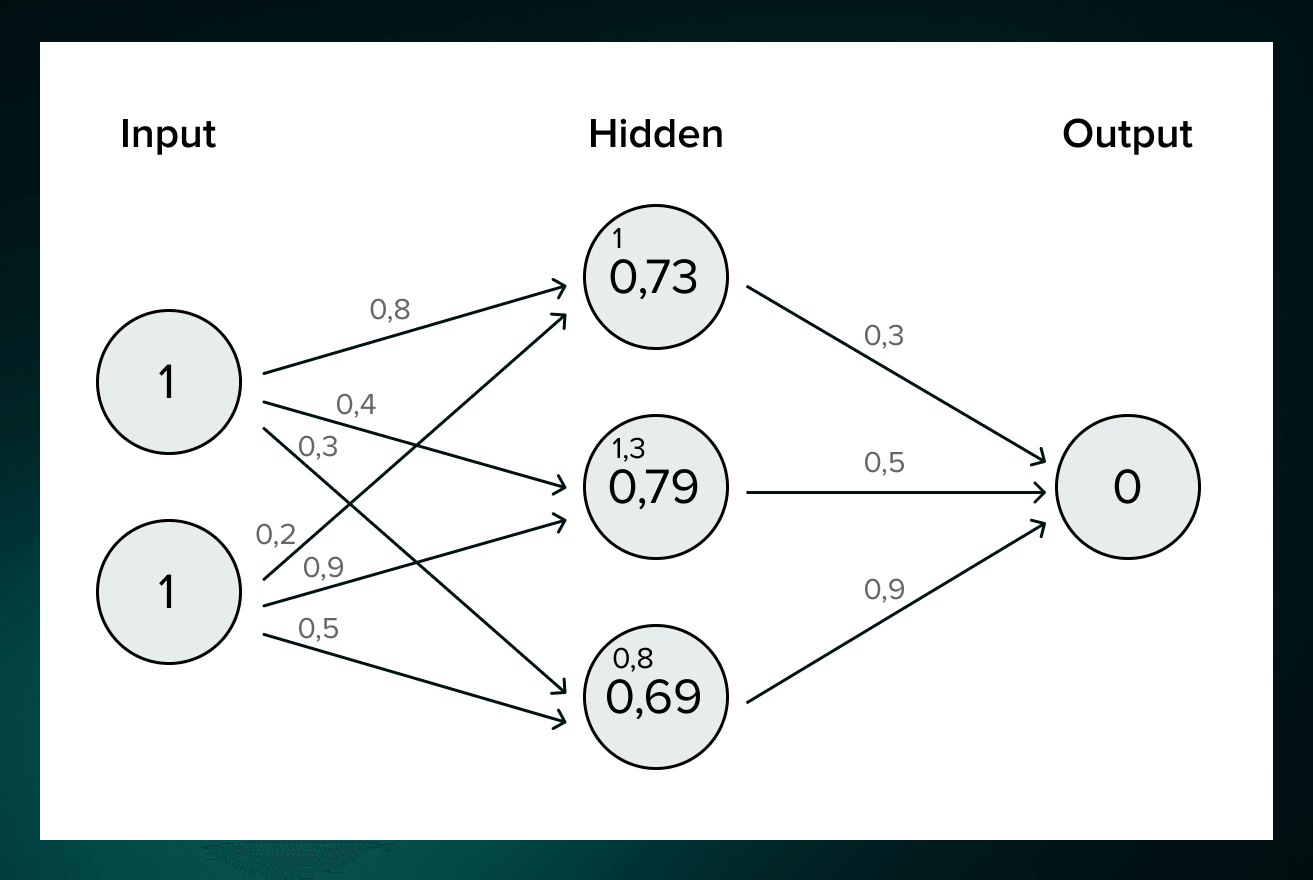
\includegraphics[width=0.5\linewidth]{graphics/network.png}
    \caption{Aufbau eines neuronalen Netzwerks}
    \label{fig:network}
\end{figure}

Damit ein Modell zuverlässig Anschlagspunkte erkennen kann, benötigt es Trainingsdaten, die korrekt klassifiziert sind. 
Während des Trainingsprozesses wird der Output des Modells mit den tatsächlichen Zielwerten verglichen, um den Verlust (Error) 
zu berechnen. Ziel ist es, diesen Verlust so gering wie möglich zu halten. Dies geschieht durch Optimierungsverfahren wie den 
Gradientenabstieg, bei dem die Ableitung der Verlustfunktion berechnet und zur Anpassung der Gewichte im Netzwerk verwendet wird.



\subsubsection{Probleme mit Machine Learning}
Künstliche Intelligenz (KI) ist ein faszinierendes und vielversprechendes Thema, bringt 
jedoch einige Herausforderungen mit sich. Eines der Hauptprobleme ist der immense Bedarf 
an qualitativ hochwertigen Daten, die oft manuell aufbereitet und annotiert werden müssen. 
Dieser Prozess ist zeitaufwendig und erfordert erhebliche personelle und technische Ressourcen.

Darüber hinaus sind KI-Systeme in der Regel äusserst rechenintensiv. Wenn solche Systeme auf
einer Baustelle eingesetzt werden sollen, ist es oft notwendig, die Berechnungen remote in 
leistungsstarken Rechenzentren durchzuführen. Dies führt nicht nur zu zusätzlichen Kosten, 
sondern auch zu potenziellen Verzögerungen durch Latenzzeiten bei der Datenübertragung.

Ein weiteres Problem besteht darin, dass die KI allein anhand von Bilddaten ohne zusätzliche 
Informationen, wie etwa den genauen Dimensionen der Anschlagspunkte, Schwierigkeiten hat, 
präzise Berechnungen für die korrekte Ausrichtung der Traverse durchzuführen.
Dies verdeutlicht die Notwendigkeit einer Kombination aus KI-gestützter Objekterkennung und 
zusätzlichen sensorischen Daten, um zuverlässige Ergebnisse zu erzielen.

\subsection{Kameras}
Um die Anschlagpunkte zuverlässig erkennen zu können, sind geeignete Kamerasysteme
erforderlich. Um zu verstehen, warum bestimmte Schritte, wie beispielsweise die 
Kalibrierung der Kamera, notwendig sind und warum es zu Ungenauigkeiten bei den 
Berechnungen zur Positionierung der Traverse kommen kann, betrachten wir in diesem 
Abschnitt die Funktionsweise und Eigenschaften von Kamerasystemen genauer.

\subsubsection{Kameraeigenschaften}
Eine Kamera kann ein Bild generieren, das insgesamt \( L \) Pixel in 
der Länge und \( H \) Pixel in der Höhe besitzt. \( L \) und \( H \) 
beschreiben hierbei die Auflösung der Kamera. Die Auflösung ist ein 
wichtiger Faktor, da sie bestimmt, wie viele Details in einem Bild 
sichtbar sind. Höhere Auflösungen ermöglichen genauere Berechnungen, 
erfordern jedoch auch mehr Rechenleistung für die Verarbeitung der 
Bilder.

Das FOV (Field of View) einer Kamera beschreibt den Bereich der Szene,
den die Kamera sehen oder aufnehmen kann. Es ist ein grundlegender 
Parameter, der angibt, wie viel von der Umgebung eine Kamera in einem 
Bild oder Video erfassen kann. Je höher das FOV, desto größer ist 
jedoch die Verzerrung, die im Bild entsteht.
Abbildung \ref{fig:fisheye} zeigt, wie eine starke Verzerrung aussieht,
die typischerweise bei Weitwinkel- oder Fisheye-Objektiven auftritt.

\begin{figure}[H]
    \centering
    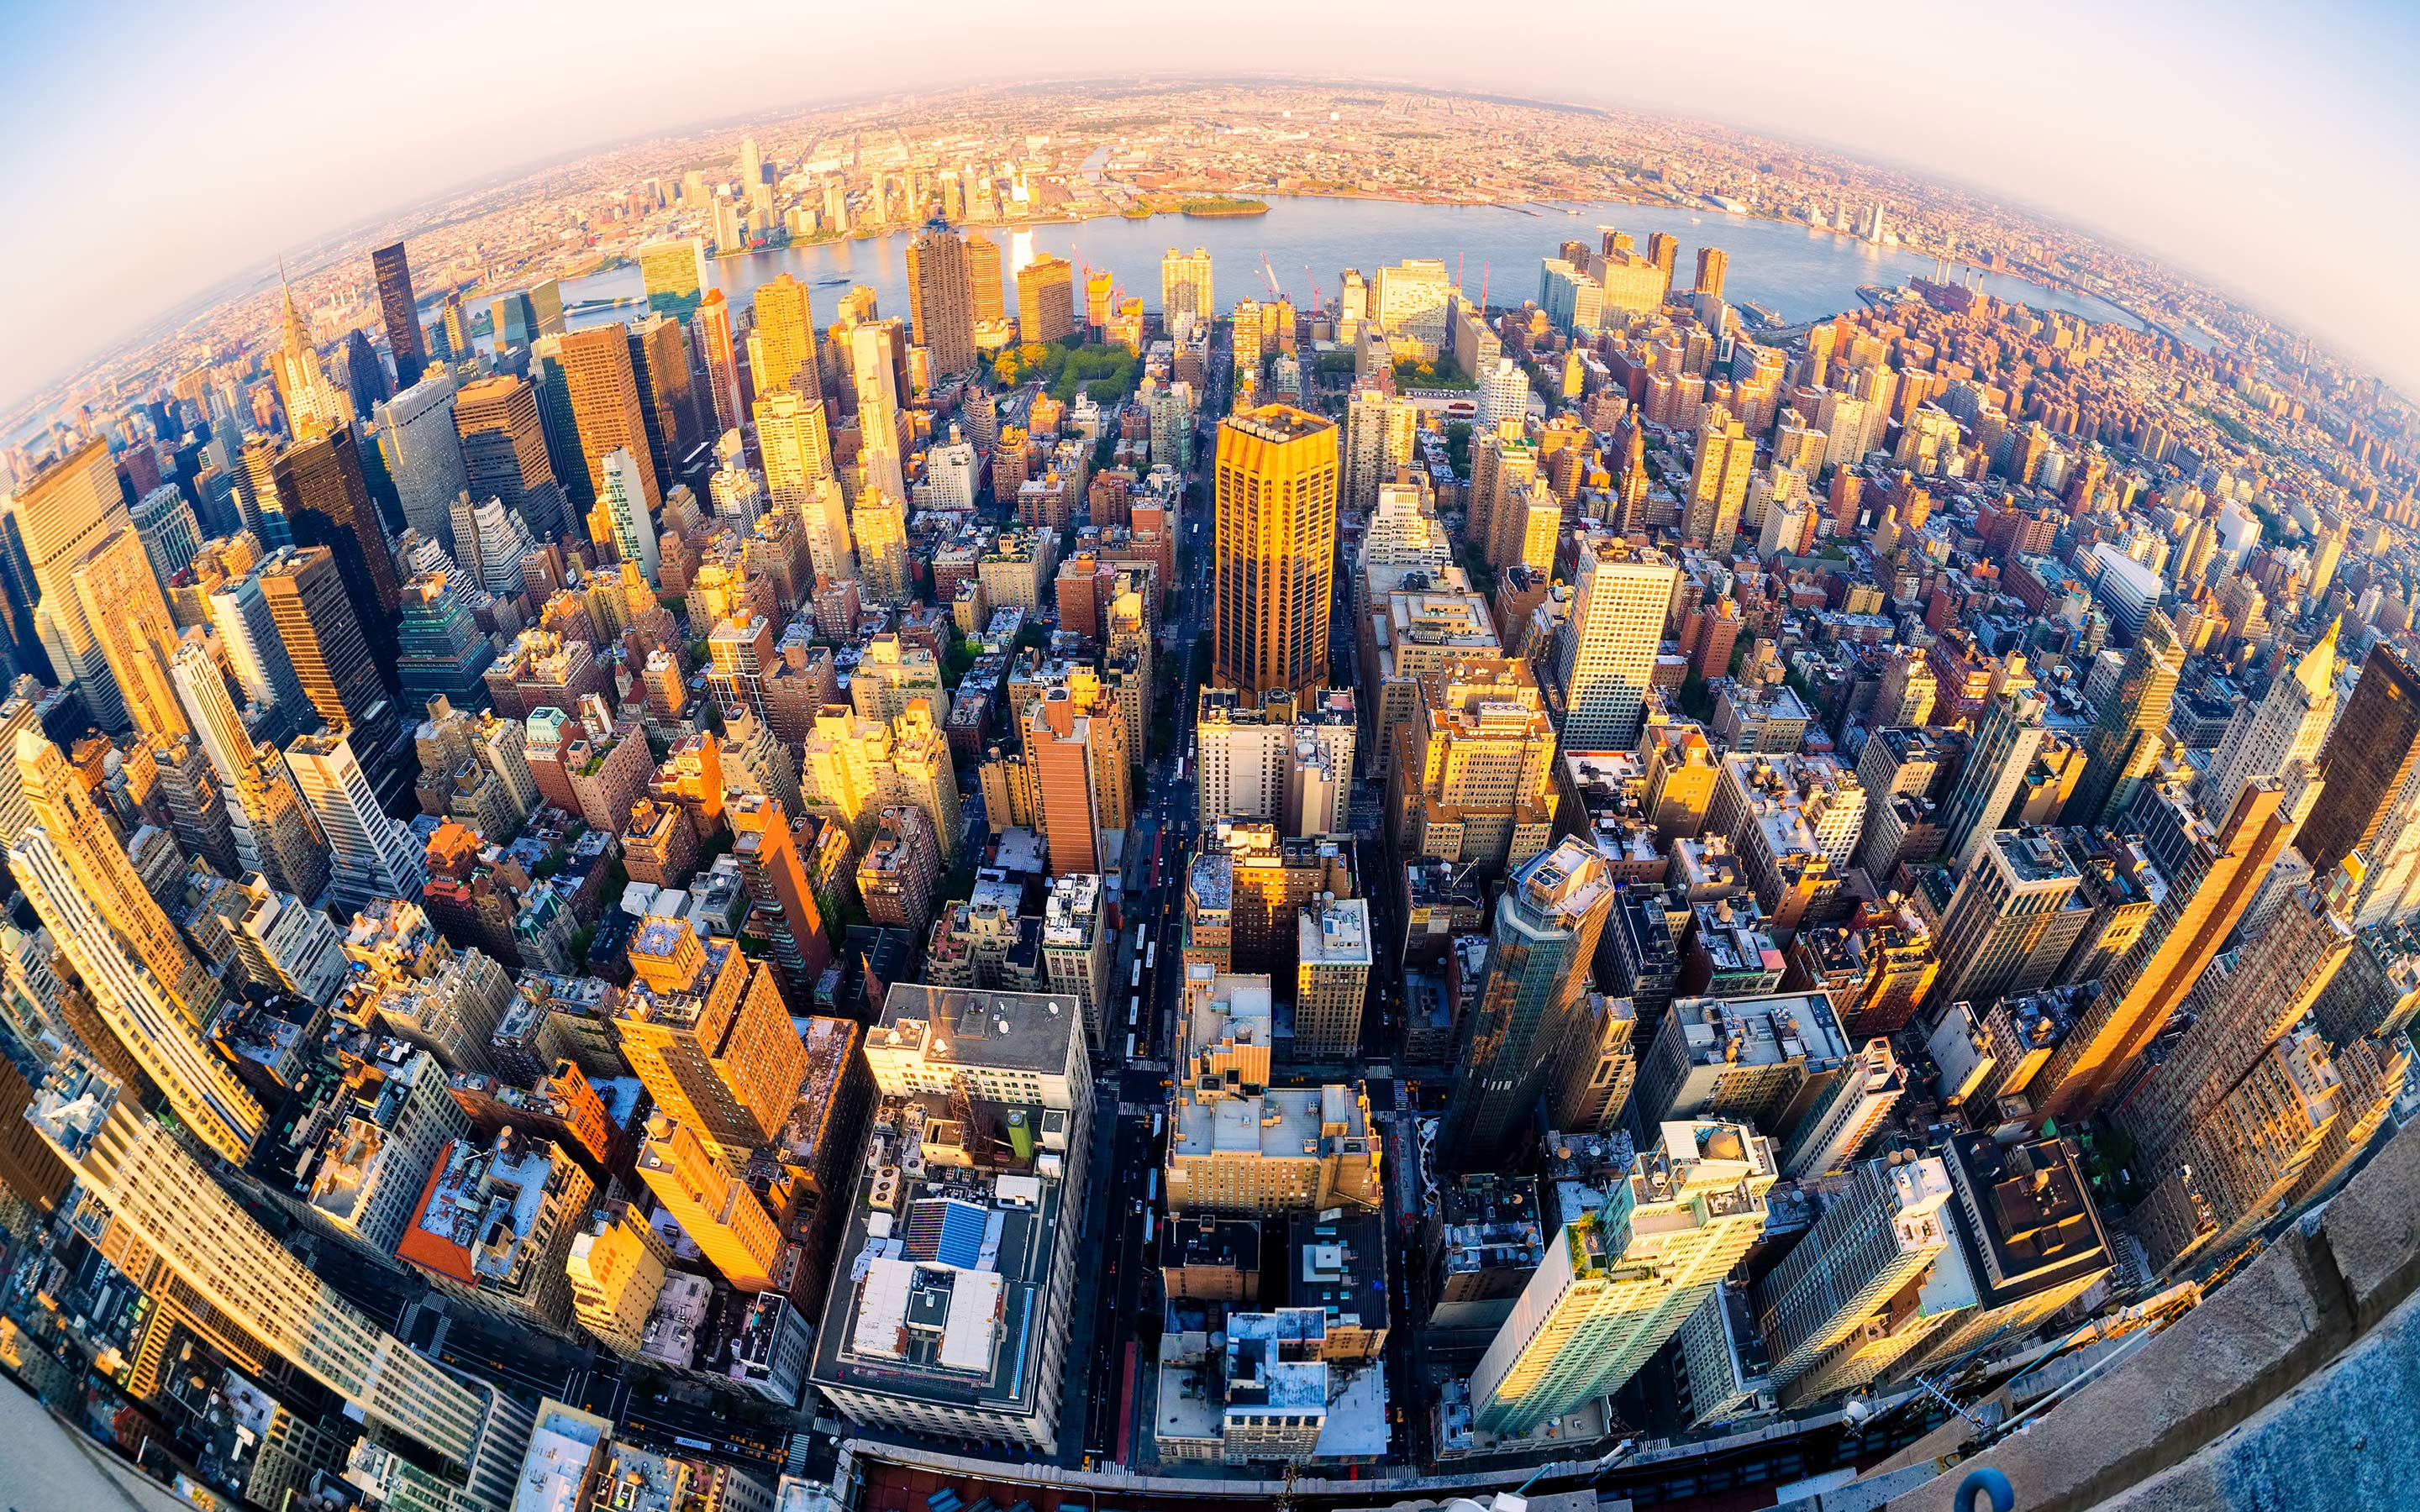
\includegraphics[width=0.5\linewidth]{graphics/fisheye.jpg}
    \caption{Beispielfoto einer starken Verzerrung}
    \label{fig:fisheye}
\end{figure}

Neben Auflösung und FOV gibt es weitere wichtige Eigenschaften, die 
bei der Auswahl und Nutzung einer Kamera berücksichtigt werden sollten:

\begin{itemize}
    \item \textbf{Bildrate (Frame Rate):} Gibt an, wie viele Bilder pro Sekunde aufgenommen werden können.
    \item \textbf{Fokus und Tiefenschärfe:} Der Fokusbereich beeinflusst, welche Bereiche des Bildes scharf dargestellt werden.
\end{itemize}


\subsubsection{Intrinsische Kalibrierung}
Verzerrungen, insbesondere an den Kanten eines Bildes, können zu Rechenfehlern 
bei der Positionierung der Traverse führen. Verzerrungen entstehen durch optische 
Abweichungen der Linse und sind besonders bei hohen FOV-Werten ausgeprägt. 
Zudem können sie die Erkennung der Anschlagpunkte erschweren, da die Form und 
Lage der Marker falsch interpretiert werden können.

Um diese Probleme zu vermeiden, muss die Kamera vor ihrem Einsatz kalibriert
werden. Die Kamerakalibrierung umfasst die Korrektur von Verzerrungen 
(z. B. radialen und tangentialen Verzerrungen) sowie die Bestimmung der 
intrinsischen Parameter der Kamera, wie:

\begin{itemize}
    \item \textbf{Brennweite} (\( f_x, f_y \)): Gibt an, wie stark die Linse das Licht bündelt.
    \item \textbf{Hauptpunkt} (\( c_x, c_y \)): Die Koordinaten des optischen Zentrums auf dem Bildsensor.
    \item \textbf{Verzerrungskoeffizienten}: Parameter, die die Stärke der Verzerrungen beschreiben.
\end{itemize}

Um eine Kamera zu kalibrieren, werden mehrere Fotos eines regelmäßigen Musters 
benötigt, beispielsweise eines Schachbretts. Die Bilder sollten aus verschiedenen 
Distanzen und Blickwinkeln aufgenommen werden, um eine möglichst breite Datenbasis 
zu schaffen. Dabei ist es wichtig die Kamera zu bewegen, während das Muster, 
beispielsweise auf einer Wand, fest positioniert bleibt.

Die Dokumentation von OpenCV \cite{opencv_calibration_tutorial} liefert praktische 
Beispiele und erklärt detailliert, wie die Kalibrierung implementiert werden 
kann.


\subsection{Vorhandene Frameworks}
OpenCV ist eine populäre Open-Source-Bibliothek für verschiedene Bildverarbeitungssoftware.
Open Source bedeutet, dass die Funktionen für jeden frei verfügbar sind. OpenCV bietet 
umfangreiche Funktionen, um AruCo-Marker zu erkennen und eine Kamerakalibration durchzuführen.
Weitere Informationen zu OpenCV finden sich auf der offiziellen Webseite unter opencv.org.

Allerdings unterstützt OpenCV keine Erkennung von AprilTags. Um diese Aufgabe zu erfüllen, verwenden 
wir stattdessen eine spezielle Ressource, die im GitHub-Repository für AprilTags bereitgestellt 
wird \cite{apriltag_github}. Dieses Repository basiert auf drei wissenschaftlichen Arbeiten 
\cite{olson2011tags} \cite{wang2016iros} \cite{krogius2019iros} und bietet eine effiziente 
und robuste Lösung zur Erkennung von AprilTags. Die Software wird unter der BSD 2-Clause License 
veröffentlicht, die eine freie Nutzung, Modifikation und Weiterverteilung unter bestimmten Bedingungen 
erlaubt. Weitere Details zur Lizenz können direkt im Repository nachgelesen werden.